\documentclass[a4paper]{article}
\usepackage[margin=1.2in]{geometry}
%\usepackage{fontspec}


%%%%lualatex on
%\usepackage{luatextra}
\usepackage{fontspec}
%Ligatures={Contextual, Common, Historical, Rare, Discretionary}
\setmainfont[Mapping=tex-text]{Linux Libertine O}
%%First draft of a research proposal

\usepackage{natbib}
\usepackage{graphicx}


\title{Research Proposal}
\author{Simon Carrignon}

\begin{document}


\subsection*{Simon Carrignon - EPNet (ERC 340828)}
\subsection*{\\PhD Research Proposal}

This PhD is fully funded and part of the Economy and Political Network project (EPNet - ERC 340828 ), whose general objective is :
\begin{quote}
	``[\ldots]to investigate the political and economical mechanisms that characterised the dynamics of the commercial trade system during the Roman Empire.''
\end{quote}
To attain this objective the project want to propose a new and innovative framework that bring together evolutionary thinking, economics, history and archaeology to study the evolution of the economical and cultural dynamics during the Roman Empire. 

Within this framework, the thesis will investigate the conditions of the emergence of a free market in a pre-industrial context. To do so we will take the Roman Empire as a case study and apply actual economical model to Mediterranean historical context in order to see if this context allow a free market to evolve or not. The study will focus on the evolution of such system, when submitted to evolutionary cultural dynamics (such as random copy or learning of economical policies, imitation of the most successful individual, \ldots).


%To test those hypothesis we want to build a model using historical and archaeological evidences as well as other model already built by economists, people from game theory, evolutionary biology and evolutionary archaeology and cultural evolution. The model will offer the possibility to test different hypothesis about the nature and the evolution of those exchange and will rest on quantitative historical and archaeological evidence to calculate and determine a degree of accuracy of this hypothesis.

The goal of the thesis is to investigate an old debate in history and archaeology, which is to understand in what extent the roman economy was a fully integrated free market economy, or a heterogeneous network of small independent economics loosely connected, knowing the predominant role and control of the Roman Empire on this economy. 
 
In the same time the thesis will illustrate the viability of bringing together economical model and cultural evolution into computer simulation in order to test hypothesis about such a complex past process that is the Roman Economy, which is difficult to study other way due to a lack of data and remaining knowledge. Cultural evolution and economical model give us ways to extrapolates those missing or erroneous data, while computer simulation allows us to integrate crucial spacial and behavioral specificities to better understand the historical process.

%To answer this problem, the main idea will be to build an Agent-based model that integrate economical hypothesis and cultural evolution assumption to study the evolution of cultural and economical exchange in the Roman Empire.

%An Agent-Based model upon which all follow experiment will be done has already been developed to serve as a theoretical proof of concept, leading to a conference presentation in (WSC ?) and is build using the Multi-Agent platform Pandora \citep{rubio2014pandora}.


The first step of the research will consist on a theoretical exploration, to understand which cultural and economical dynamics lead to which type of economical system (centralized economy, free market or heterogeneous economy) given different geographical, demographics and political context.

In a second time, the thesis will use evolutionary archaeological tools and all available data to choose the more probable scenario among those previously explored and review them if needed.

To succeed in those tasks the PhD will be co-supervised by Sergí Valverde from the Complex System Lab and Xavier Rubio from the Barcelona Supercomputing Center, thus it will benefit the expertise of their associated lab on modeling and analysing complex adaptive systems. Moreover it will rely on all team already engaged in the EPNet project, who are the rest of the team in the Barcelona Supercomputer Center, with whom the theoretical model is ale rad under development, the CEIPAC  laboratory, specialised in Ancient History and the Roman Empire and the PhysComp laboratory specialised in network an big data analysis.

%In the following paragraphs we will quickly argue why we choose Agent-Based Modeling and how we will position it in regards to evolutionary process and evolutionary thinking. Then we will propose some economical approach that we think promising in our context and with our approach, and we will finish explaining how we will articulate the model with archaeological and historical studies.
%
%
%\section{Simulation and Agent Based Modelling}
%Since the 90s, the use of Simulation and Agent-Based Modeling (ABM) in Science is inexorably growing. One can observe that not only by the amount of published papers using ABM, but moreover through the different fields of study those publication encompass, ranging from Ecology \citep{grimm2005individual} to Social Sciences in general \citep{epstein1996growingartificialsocietiessocialsciencefromthebottomup} with Economy \citep{tesfatsion2006agentbasedcomputationaleconomicsaconstructiveapproachtoeconomictheory} or Archaeology \citep{wurzer2015agentbasedmodelingandsimulationinarchaeology} in particular.
%
%For each discipline, Agent-Based Model will bring specific advantage over traditional methods. Without looking to all of those advantage we will present some of them generally admitted. First ABM allow to precisely define the historical and the environmental context where studied processes are taking place. Moreover, it allows to integrate in a pretty direct way knowledge from different fields. This knowledge could be integrated at the agent's level, for example when defining the agent's cognitive or physiological abilities \citep{chen2012varietiesofagentsinagentbasedcomputationaleconomicsahistoricalandaninterdisciplinaryperspective}, or during the environmental design, for instance by situated the agents in a geographically and historically consistent environment.
%
%ABM is also perfectly suited to study process that evolve through time. It allow no only to look at global trends but also to follow the whole evolutionary trajectory of the system and each of this constituent, which is often far more important than the final output of the process.
%
%We will now see why we think this is important to be able to study such evolutionary process in our context.
%
%
%\section{Evolutionary Process, Darwinism and Evolutionary approach}
%
%By evolutionary process we mean all systems that evolve through time under the action of reproduction/replication, variation and inheritance mechanisms. Since 1859, the Theory of Evolution of Darwin, also called Darwinism (or neo-Darwinism in is updated actual form), provide a powerful approach to study such processes\nocite{darwin1859originspeciesbymeansnaturalselectionorpreservationfavouredracesstrugglelife}.
%%During the 20th century, the Darwin's approach has been successfully update by the Modern Synthesis \citep{huxley1942evolution} and now by what is often called neo-Darwinism.
%In our perspective, we will prefer to use ``Evolutionary Approaches'', or ``Evolutionary Thinking'', instead of Darwinism, to speak about ways to study evolutionary process build upon Darwinism but including a wider kind of process. Those processes could involved systems with more ``unorthodox\footnote{From a Darwinian perspective}'' entities or mechanisms of replication, variation and inheritance ; and so could be driven by other force than the Natural Selection as initially described by Darwin\footnote{Actually neo-Darwinism already include more and more of those unorthodox mechanism, like random drift or non-Mendelian inheritance, but it could still exclude evolutionary processes that are interesting for this present work. For a more permissive point of view, an interesting discussion and a good framework that unify those unorthodox systems, one can look at \cite{godfrey2009darwinian}}.
%
%By itself and given this definition, the study of evolutionary processes can encompass a wide range of problems, from totally different scientific horizons and studied by (sometimes) vigorously opposed school of thought. And if the Darwin's Evolutionary Theory is widely admitted since more than half a century as the more accurate framework able to unify all biological science\footnote{One could think about the famous title widely cited of the 1975 Dobzhansky essay : \emph{``Nothing in Biology Makes Sense Except in the Light of Evolution''}} ; people trying to pushed forward Evolutionary approach as a framework able to unify all the sciences of life -- in a wide sense of ``science that study living things'', ranging from biology to sociology, has always encountered difficulty to do so.
%
%One of the major problem faced by this agenda that want to apply evolutionary thinking to a wider range of problem\footnote{This idea of using evolutionary theory could in fact be tracked back to \cite{darwin1871thedescentofman} himself but are maybe more explicitly expressed by people like \cite{spencer1864theprinciplesofbiology}}, is that it had often lead to misleading interpretations of the evolutionary mechanisms in action and is deeply loaded with tragic political derives, eugenics and human determinism. Without enter into the details of the history and debates around those problem, we will follow \cite{shennan2002genes} and take as granted :
%\begin{quote}
%	[\ldots] the power of the [Evolutionary] approach in explaining many of the patterns we observe in the past, and the fact that Darwinian approaches\footnote{Shennan use Darwinian approach where us prefere Evolutionary approach as told before, to take some distance we pure, more restrictive, Darwinian Theories.}  do not necessarily have the dubious implications that many, if not most, archaeologists [and indeed lot of people from fields not concern with evolutionary biology] believe; in particular they are much more about importance of historical trajectories, situationally appropriate strategies and differences in interests than differences in human capacity.\\
%	\cite[p. 14]{shennan2002genes}
%\end{quote}
%Indeed people studying Cultural Evolution \citep{mesoudi2015culturalevolutionareviewoftheoryfindingsandcontroversies}, Evolutionary Computation \citep{eiben03introductiontoevolutionarycomputing}, Evolutionary Robitics \citep{nolfi00evolrobobiolintetechselfmach} or using what is something called ``Darwinian Archaeology''\citep{shennan2002genes} or ``Evolutionary Archaeology'' have already successfully shown that evolutionary approaches provides a lot of tool that could help to study a wide range of different problems, and it's those tools that we want to use.  
%
%Moreover evolutionary biology is a complex and still changing field, far from what it was after Darwin's books. Thus when speaking about apply evolutionary approach to something different than biological entities, it's more about embracing a complex and not fixed way of thinking, of using quantitative tools, visualizing methods and epistemological approaches to study complex evolving \& adaptive system deeply embodied into an environmental and historical context where all compound of the system interact together ; than to speculate about the philosophical implication of applying general ideas on almost everything, as Spencer and his followers could have been done.
%
%In another hand, core question in evolutionary biology remains subject to debate. Among them, the  nature and the type of explanation that evolutionary biology can produce or need to follow remain complex. As remarked by the Physicist Nobel Delbrück :
%\begin{quote}
%	[\ldots] there are no ``absolute phenomena'' in biology. Everything is time bound and space bound. \\
%	(Delbrück~1952)
%\end{quote}
%which lead philosophers of science, following \cite{gould1989wonderfullife} and his contingency concept, to think Evolutionary Biology as more close to an historical science than to Physics \cite{beatty1995theevolutionarycontingencythesis}.Indeed, to understand the evolutionary trajectory of biological systems, one cannot only look at a population level to extract law from the dynamics of the population, as a physicist could infer laws from a corps without looking to the molecule composing it. In a biological context, individual evolve and adapt themselves to their environment and when doing so, they modify this environment. Those modifications in turn lead to the modification of the evolution and of the adaptive dynamics of the individual, thus creating an always changing historical context that one need to know in order to understand general pattern that could appear at a more general level. One could derive the Hardy Weinberg equilibrium from the Mendel Law, and works on the allele's population dynamic with that. But those equations doesn't say anything about the adaptive value of the Mendel laws at the individual level in the current individual context. They could be unadaptive, and so subject to evolutionary change. In that case all dynamics coined by the HW equilibrium could be false. As says \cite{lomnicki1978individualdifferencesbetweenanimalsandthenaturalregulationoftheirnumbers}, equation could lead ``theoretical population biology into a blind alley''. We think that ABM is a way to avoid that.
%
%%Without embracing the whole philosophical implication of such proposition, we think it's a good framework arguing in favor of the use of similar tools to study different fields with similar evolutionary concerns.
%
%Given all that we think ABM is one of the most efficient way to 
%\begin{itemize}
%	\item Integrate concepts from different fields that use Evolutionary Approaches and that could bring interesting tools for the project (i.e. cultural evolution model, ecological model\ldots) ,
%	\item Catch all the properties associated with evolutionary processes seen as complex adaptive system deeply embodied in historical and environmental context.
%\end{itemize}
%
%
%\section{Economy and Ancient Economy}
%
%Since \cite{smith1776wealthofnation} and is  Wealth of the Nation, modern economists have developed a lot of different theories to describe how economics work in our societies ; and today economics is a well established science laying on strong mathematical roots. 
%
%But mainstream modern economy (often called neoclassical economy) is heavily critiqued by the economist themselves. Some argues that neoclassical economy release on assumption that simplify the behavior of the agents that compose the economy as acting optimally. People like \cite{lebaron2008modelingmacroeconomiesasopenendeddynamicsystemsofinteractingagents} advance that it should not be taken as granted and to understand macro-economical dynamics, 
%\begin{quote}
%	[\ldots] would seem to require a systematic exploration of the intricate feedback loops connecting micro behaviors, interaction patterns, and macro regularities as observed in real-world economies.\\
%	(\emph{ibid})
%\end{quote}
%
%They propose Agent-Base Modeling, termed Agent-Base Computational Economics (ACE) in this context, as a solution to deal with such problems. 
%
%From an historical point of view, even if always more and more historian and economists urge to apply traditional neo-classical model or more heterodox one to test on which extend they could correspond to ancient economy, concrete implementation of those idea remains anecdotal. We think that ACE is the perfect tool to fill this gap.
%
%In the more precise case of the Roman Empire, the debate on whether or not its economy was subject to a free market is still active (\cite{temin2013theromanmarketeconomy}). In fact the precise nature of this economy is still uncertain. Most of 
%
%The idea to apply New Institutional Economics to understand it seems to be more and more appealing \citep{bang2009ancienteconomy,verboven2015theknightwhosaynie} when in the same time \cite{grantham2015reserarchequilib} propose the \cite{diamond1982aggregatedemandmanagementinsearchequilibrium}research equilibrium model as more adapted to the Roman Economy, while \cite{poblome2013moneymakespotterygoround}  suggest that an oligopoly approach \citep{vives2001oligopoly} could help to understand such trade dynamics as the olive oil market. The thesis will focus on some of those model and try to apply it  to precise subpart of the Roman Empire, given the other research of the partner in the EPNet project.
%
%Furthermore, Historians and Archaeologists warn us of the danger to forget to include political and cultural context when looking at such economical dynamics. Some of them argue that today's market economics is now detached from this and working on fully decentralized and optimal agent. In fact doing so they join the ACE critics, thus given more weight to the use of Agent-Based Modelling that will integrate knowledge from different field of study, as done by people studying Evolutionary Process in general ( cf section 3).
%
%
%\section{Historical and Archaeological Validation}
%
%Whereas a model by itself can bring some theoretical knowledge or not is matter of discussion, but it any case it remains subject to an infinity of possible meaningless (historical, biological, cultural\ldots) interpretations if we do not confront it to (historical, biological, cultural\ldots) data. To encompass this obstacle, and as a part of the EPNet Project, this thesis will rely on massive data from different partners of the project. 
%
%From those data --that are mainly about trade and cultural exchange, military campaign and good productions during the Roman Empire, one of the main objective of the project will be, conjointly with the historian and archaeologist experts and given the available knowledge, to draw precise questions that the model will help to explore. This question will allow to test different hypothesis about the nature of the ancient economy and need to insure that, given the available data and historical knowledge, solid statistical method could be use to interpret the results and the validity of the model.
%
%In this thesis we will follow hypothesis made by some historians, archaeologists and ancient economists (Remesal, Poblome\ldots) that think that the huge logistic, the big amount of supply and food needed to be sent by the Empire to maintain its troops all around its territory, offer the perfect context, with a huge trade network and production infrastructures, to allow free market to evolve throughout the empire.  
%The idea is to explore how react an heterogeneous economy such as the Roman one under different condition in an evolutionary perspective. What are the condition (cultural, political, geographical, demographics) that need to be met in order that a fully integrated, decentralized, free market, evolve. This to provide theoretical argument to answer  the question raised by Wilson et al to know if Roman provinces could be seen 
%\begin{quote}
%	as part of a single economy or economic system, or simply as a number of small ‘economies’ linked to a greater or lesser degree.
%\end{quote}
%
%Furthermore, using archaeological and historical data data brings new problems that are less often found in evolutionary study like those done in Biology (for instance) :  the archaeological and historical record are partial and subject to multiple sources of bias. A lot of information, useful (even mandatory) to understand the past economical process, are lacking or have to used with caution. They could have been destructed by time, not stored in anyway by the actor of the past process or even badly interpreted by archaeologists or historians and so on. When building such a model one need to take it into account. Hopefully a lot of literature already exist about that kind of problem in Evolutionary Archaeology (Madsen 2012, Premo 2014), and ABM gives use way to deal with it and to model those bias \citep{rubiocampillo2012simulatingarchaeologist}. Indeed it allow us to model \emph{the evolution of the past process} (here the Ancient Economy), as well as \emph{the record of this evolution} and how this record deteriorate through time, as well as to model \emph{the discovery of this record}.
%
%
%
%\section{Conclusion}
%
%Using data coming from advanced research in archaeology and history done by the CEIPAC laboratory, the PhD will focused on building computer simulation where economical model, evolutionary process and historical knowledge are bind, to study the evolution of the Economy in the Roman Empire. The goal of the thesis is to explore the historical context allowing the evolution or not of a decentralized, fully integrated free market and to compare this context and its evolution with what we know about the Roman Empire market. Moreover, this study will  show the suitability of the approach to study past economy as a Complex Adaptive System using computer simulation.
%
%
%
%\bibliographystyle{apalike}
%\bibliography{/home/scarrign/Documents/biblio/bib/phd,/home/scarrign/Documents/biblio/bib/memoireLophiss}  
	\begin{center}
		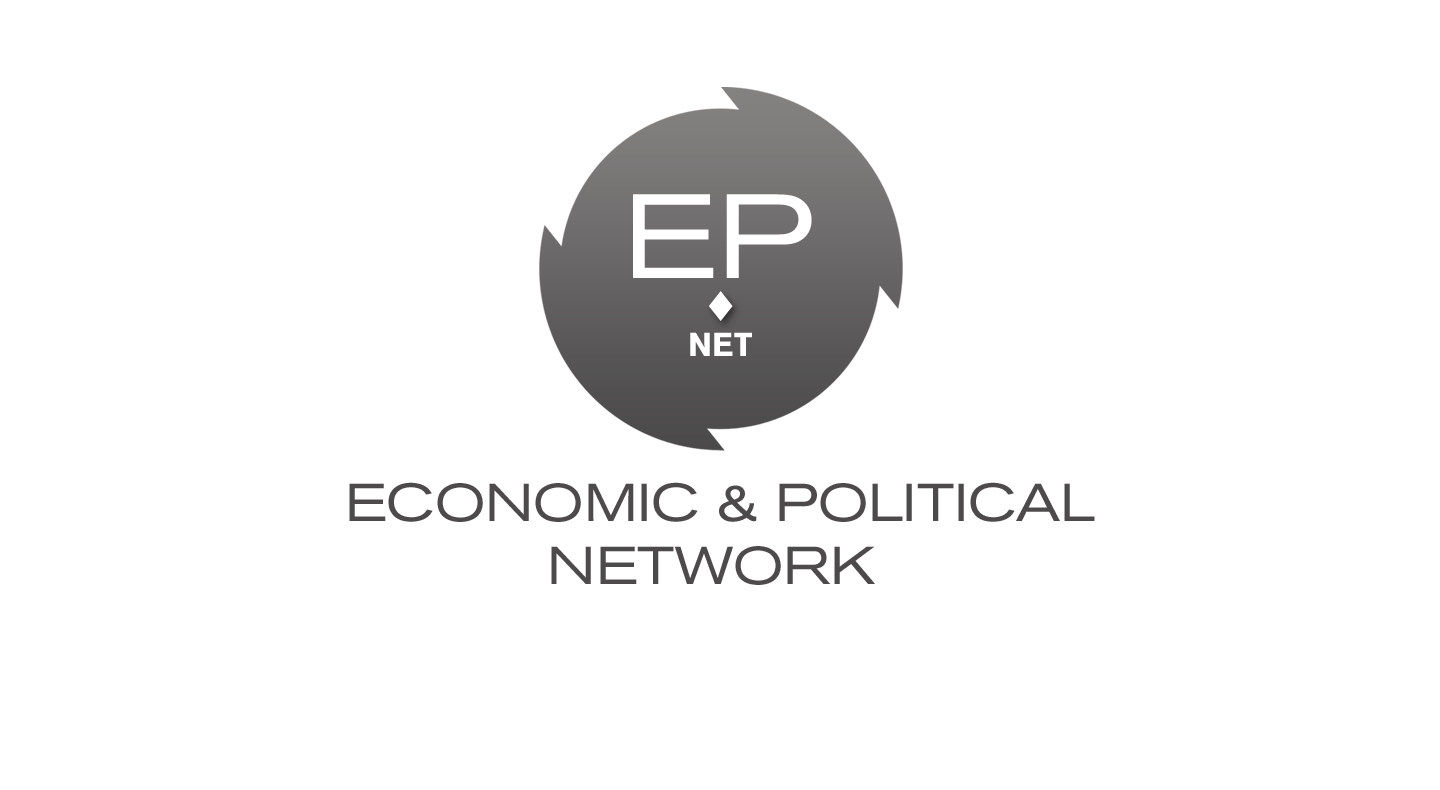
\includegraphics[width=7cm]{logo}
	\end{center}
\end{document}
